%!TEX root = ../iotpaper.tex

%~~~~~~~~~~~~~~~~~~~~~~~~~~~~~~~~~~~~~~~~~~~~~~~~~~~~~~~~~~~~~~~


\section{Simultaneous Gestures \\ Experiments}
\label{sec:Simultaneous}
In the Simultaneous Gestures model, we assume the pebble smartwatch is the verifier, an iPhone is the legitimate prover, and the other iPhone is the malicious attacker. Three devices start and end each authentication attempt at the same time. As an proof of concept, the prover and verifier are held together with all axes of accelerometers are correctly aligned. The attacker observes this authentication and tries to copy the gesture. Successful attackers could potentially hijacking the current authentication or a replay the data later if the legitimate user tends to use the same gesture for authentication. Henry and Gino collect data for 4 gestures, and each gesture was tested with 10 attempts. The gestures are gesture 5, 7, 11, 17 in \autoref{tab:GestureTable}. Ideally, the prover should be authenticated because it moves together with the legitimate prover and attacker should be denied. For this model, we leave setting the threshold for authentication to future work and only look at the raw distance values. We hypothesize that the \gls{DTW} distance for the legitimate prover should be lower than the attacker for all attempts.

 \begin{figure*}[!t]
% 	\vspace{-1.5em}
    	\centering
 	\subfloat[Gesture \#5 ]{
 	\centering
 	\tikzquarter
		\input{../../Data/plots/simultaneousplots/numeight.tikz}
 		 \label{fig:s5}}
 	\subfloat[Gesture \#7]{
 	\centering
 	\tikzquarter
		\input{../../Data/plots/simultaneousplots/zi.tikz}
 		 \label{fig:s7}}
 	\subfloat[Gesture \#11]{
 	\centering
 	\tikzquarter
		\input{../../Data/plots/simultaneousplots/ru.tikz}
 		 \label{fig:s11}}
	\subfloat[Gesture \#17]{
 	\centering
 	\tikzquarter
		\input{../../Data/plots/simultaneousplots/box.tikz}
 		 \label{fig:s17}}
 	\caption{DTW Distance from both the attacker and the legitimate prover to verifier for the Simultaneous Gestures model. Data is separated by gestures, and each data point is a raw attempt.}
 	\label{fig:SimultaneousDistanceMatrixPlot}
 \end{figure*}

%\begin{figure}[!tb]
%\centering
%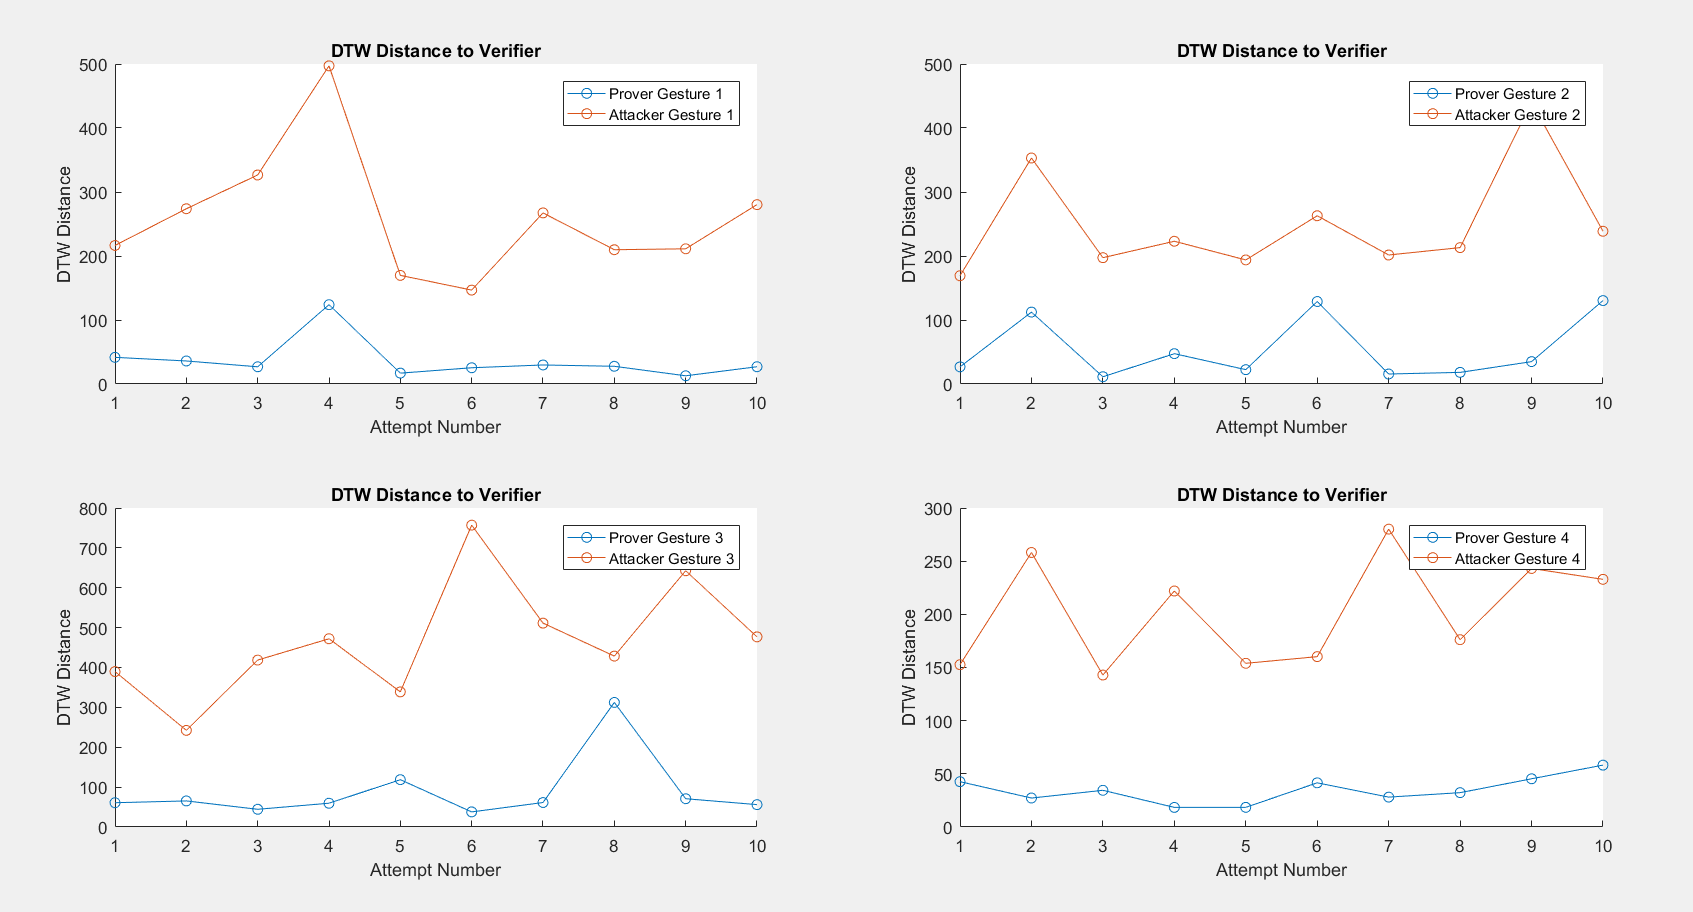
\includegraphics[width= \linewidth]{./figures/simultaneous_model_distance_matrix.png}
%\caption{DTW Distance from both attacker and prover to verifier, separated by gestures.}
%\label{fig:SimultaneousDistanceMatrixPlot}
%\end{figure}

The results for all attempts are plotted in \autoref{fig:SimultaneousDistanceMatrixPlot}. Most distance from the legitimate prover to the verifier are less than 100 and only 5 samples have distance larger than 100. This shows that when two devices are held together, it is easy to get low distance result between them and this can be exploited for pairing small devices. The distance between the attacker and the legitimate prover are all larger than 100 and most of them are more then 200. Compared with the distance result of prover, the distance of attacker is always at least 100 larger than that. It is easy to differentiate the attacker from the prover, so that our Simultaneous Gestures model is a promising authentication mechanism. 






%~~~~~~~~~~~~~~~~~~~~~~~~~~~~~~~~~~~~~~~~~~~~~~~~~~~~~~~~~~~~~~~
 

